% Options for packages loaded elsewhere
\PassOptionsToPackage{unicode}{hyperref}
\PassOptionsToPackage{hyphens}{url}
\PassOptionsToPackage{dvipsnames,svgnames,x11names}{xcolor}
%
\documentclass[
  10pt,
]{article}

\usepackage{amsmath,amssymb}
\usepackage{iftex}
\ifPDFTeX
  \usepackage[T1]{fontenc}
  \usepackage[utf8]{inputenc}
  \usepackage{textcomp} % provide euro and other symbols
\else % if luatex or xetex
  \usepackage{unicode-math}
  \defaultfontfeatures{Scale=MatchLowercase}
  \defaultfontfeatures[\rmfamily]{Ligatures=TeX,Scale=1}
\fi
\usepackage{lmodern}
\ifPDFTeX\else  
    % xetex/luatex font selection
    \setmainfont[]{Arial}
\fi
% Use upquote if available, for straight quotes in verbatim environments
\IfFileExists{upquote.sty}{\usepackage{upquote}}{}
\IfFileExists{microtype.sty}{% use microtype if available
  \usepackage[]{microtype}
  \UseMicrotypeSet[protrusion]{basicmath} % disable protrusion for tt fonts
}{}
\makeatletter
\@ifundefined{KOMAClassName}{% if non-KOMA class
  \IfFileExists{parskip.sty}{%
    \usepackage{parskip}
  }{% else
    \setlength{\parindent}{0pt}
    \setlength{\parskip}{6pt plus 2pt minus 1pt}}
}{% if KOMA class
  \KOMAoptions{parskip=half}}
\makeatother
\usepackage{xcolor}
\setlength{\emergencystretch}{3em} % prevent overfull lines
\setcounter{secnumdepth}{5}
% Make \paragraph and \subparagraph free-standing
\makeatletter
\ifx\paragraph\undefined\else
  \let\oldparagraph\paragraph
  \renewcommand{\paragraph}{
    \@ifstar
      \xxxParagraphStar
      \xxxParagraphNoStar
  }
  \newcommand{\xxxParagraphStar}[1]{\oldparagraph*{#1}\mbox{}}
  \newcommand{\xxxParagraphNoStar}[1]{\oldparagraph{#1}\mbox{}}
\fi
\ifx\subparagraph\undefined\else
  \let\oldsubparagraph\subparagraph
  \renewcommand{\subparagraph}{
    \@ifstar
      \xxxSubParagraphStar
      \xxxSubParagraphNoStar
  }
  \newcommand{\xxxSubParagraphStar}[1]{\oldsubparagraph*{#1}\mbox{}}
  \newcommand{\xxxSubParagraphNoStar}[1]{\oldsubparagraph{#1}\mbox{}}
\fi
\makeatother

\usepackage{color}
\usepackage{fancyvrb}
\newcommand{\VerbBar}{|}
\newcommand{\VERB}{\Verb[commandchars=\\\{\}]}
\DefineVerbatimEnvironment{Highlighting}{Verbatim}{commandchars=\\\{\}}
% Add ',fontsize=\small' for more characters per line
\usepackage{framed}
\definecolor{shadecolor}{RGB}{241,243,245}
\newenvironment{Shaded}{\begin{snugshade}}{\end{snugshade}}
\newcommand{\AlertTok}[1]{\textcolor[rgb]{0.68,0.00,0.00}{#1}}
\newcommand{\AnnotationTok}[1]{\textcolor[rgb]{0.37,0.37,0.37}{#1}}
\newcommand{\AttributeTok}[1]{\textcolor[rgb]{0.40,0.45,0.13}{#1}}
\newcommand{\BaseNTok}[1]{\textcolor[rgb]{0.68,0.00,0.00}{#1}}
\newcommand{\BuiltInTok}[1]{\textcolor[rgb]{0.00,0.23,0.31}{#1}}
\newcommand{\CharTok}[1]{\textcolor[rgb]{0.13,0.47,0.30}{#1}}
\newcommand{\CommentTok}[1]{\textcolor[rgb]{0.37,0.37,0.37}{#1}}
\newcommand{\CommentVarTok}[1]{\textcolor[rgb]{0.37,0.37,0.37}{\textit{#1}}}
\newcommand{\ConstantTok}[1]{\textcolor[rgb]{0.56,0.35,0.01}{#1}}
\newcommand{\ControlFlowTok}[1]{\textcolor[rgb]{0.00,0.23,0.31}{\textbf{#1}}}
\newcommand{\DataTypeTok}[1]{\textcolor[rgb]{0.68,0.00,0.00}{#1}}
\newcommand{\DecValTok}[1]{\textcolor[rgb]{0.68,0.00,0.00}{#1}}
\newcommand{\DocumentationTok}[1]{\textcolor[rgb]{0.37,0.37,0.37}{\textit{#1}}}
\newcommand{\ErrorTok}[1]{\textcolor[rgb]{0.68,0.00,0.00}{#1}}
\newcommand{\ExtensionTok}[1]{\textcolor[rgb]{0.00,0.23,0.31}{#1}}
\newcommand{\FloatTok}[1]{\textcolor[rgb]{0.68,0.00,0.00}{#1}}
\newcommand{\FunctionTok}[1]{\textcolor[rgb]{0.28,0.35,0.67}{#1}}
\newcommand{\ImportTok}[1]{\textcolor[rgb]{0.00,0.46,0.62}{#1}}
\newcommand{\InformationTok}[1]{\textcolor[rgb]{0.37,0.37,0.37}{#1}}
\newcommand{\KeywordTok}[1]{\textcolor[rgb]{0.00,0.23,0.31}{\textbf{#1}}}
\newcommand{\NormalTok}[1]{\textcolor[rgb]{0.00,0.23,0.31}{#1}}
\newcommand{\OperatorTok}[1]{\textcolor[rgb]{0.37,0.37,0.37}{#1}}
\newcommand{\OtherTok}[1]{\textcolor[rgb]{0.00,0.23,0.31}{#1}}
\newcommand{\PreprocessorTok}[1]{\textcolor[rgb]{0.68,0.00,0.00}{#1}}
\newcommand{\RegionMarkerTok}[1]{\textcolor[rgb]{0.00,0.23,0.31}{#1}}
\newcommand{\SpecialCharTok}[1]{\textcolor[rgb]{0.37,0.37,0.37}{#1}}
\newcommand{\SpecialStringTok}[1]{\textcolor[rgb]{0.13,0.47,0.30}{#1}}
\newcommand{\StringTok}[1]{\textcolor[rgb]{0.13,0.47,0.30}{#1}}
\newcommand{\VariableTok}[1]{\textcolor[rgb]{0.07,0.07,0.07}{#1}}
\newcommand{\VerbatimStringTok}[1]{\textcolor[rgb]{0.13,0.47,0.30}{#1}}
\newcommand{\WarningTok}[1]{\textcolor[rgb]{0.37,0.37,0.37}{\textit{#1}}}

\providecommand{\tightlist}{%
  \setlength{\itemsep}{0pt}\setlength{\parskip}{0pt}}\usepackage{longtable,booktabs,array}
\usepackage{calc} % for calculating minipage widths
% Correct order of tables after \paragraph or \subparagraph
\usepackage{etoolbox}
\makeatletter
\patchcmd\longtable{\par}{\if@noskipsec\mbox{}\fi\par}{}{}
\makeatother
% Allow footnotes in longtable head/foot
\IfFileExists{footnotehyper.sty}{\usepackage{footnotehyper}}{\usepackage{footnote}}
\makesavenoteenv{longtable}
\usepackage{graphicx}
\makeatletter
\newsavebox\pandoc@box
\newcommand*\pandocbounded[1]{% scales image to fit in text height/width
  \sbox\pandoc@box{#1}%
  \Gscale@div\@tempa{\textheight}{\dimexpr\ht\pandoc@box+\dp\pandoc@box\relax}%
  \Gscale@div\@tempb{\linewidth}{\wd\pandoc@box}%
  \ifdim\@tempb\p@<\@tempa\p@\let\@tempa\@tempb\fi% select the smaller of both
  \ifdim\@tempa\p@<\p@\scalebox{\@tempa}{\usebox\pandoc@box}%
  \else\usebox{\pandoc@box}%
  \fi%
}
% Set default figure placement to htbp
\def\fps@figure{htbp}
\makeatother
% definitions for citeproc citations
\NewDocumentCommand\citeproctext{}{}
\NewDocumentCommand\citeproc{mm}{%
  \begingroup\def\citeproctext{#2}\cite{#1}\endgroup}
\makeatletter
 % allow citations to break across lines
 \let\@cite@ofmt\@firstofone
 % avoid brackets around text for \cite:
 \def\@biblabel#1{}
 \def\@cite#1#2{{#1\if@tempswa , #2\fi}}
\makeatother
\newlength{\cslhangindent}
\setlength{\cslhangindent}{1.5em}
\newlength{\csllabelwidth}
\setlength{\csllabelwidth}{3em}
\newenvironment{CSLReferences}[2] % #1 hanging-indent, #2 entry-spacing
 {\begin{list}{}{%
  \setlength{\itemindent}{0pt}
  \setlength{\leftmargin}{0pt}
  \setlength{\parsep}{0pt}
  % turn on hanging indent if param 1 is 1
  \ifodd #1
   \setlength{\leftmargin}{\cslhangindent}
   \setlength{\itemindent}{-1\cslhangindent}
  \fi
  % set entry spacing
  \setlength{\itemsep}{#2\baselineskip}}}
 {\end{list}}
\usepackage{calc}
\newcommand{\CSLBlock}[1]{\hfill\break\parbox[t]{\linewidth}{\strut\ignorespaces#1\strut}}
\newcommand{\CSLLeftMargin}[1]{\parbox[t]{\csllabelwidth}{\strut#1\strut}}
\newcommand{\CSLRightInline}[1]{\parbox[t]{\linewidth - \csllabelwidth}{\strut#1\strut}}
\newcommand{\CSLIndent}[1]{\hspace{\cslhangindent}#1}

\usepackage{booktabs}
\usepackage{longtable}
\usepackage{array}
\usepackage{multirow}
\usepackage{wrapfig}
\usepackage{float}
\usepackage{colortbl}
\usepackage{pdflscape}
\usepackage{tabu}
\usepackage{threeparttable}
\usepackage{threeparttablex}
\usepackage[normalem]{ulem}
\usepackage{makecell}
\usepackage{xcolor}
% Paquetes necesarios
\usepackage{amsmath}
\usepackage{amssymb}
\usepackage{graphicx}
\usepackage{fancyhdr}
\usepackage{geometry}

% Configuración de márgenes
\geometry{
  a4paper,
  left=2.5cm,
  right=2.5cm,
  top=1.5cm,
  bottom=2.5cm,
  includeheadfoot
}

% Configuración de encabezado y pie de página
\pagestyle{fancy}
\fancyhf{} % Limpia encabezado y pie de página

% Encabezado
\lhead{
\includegraphics[height=1.5cm]{logo.png}} % Logo en el encabezado
\chead{}
\rhead{\small Clase reproducibilidad y replicabilidad.}

% Ajuste de separación entre encabezado y contenido
\setlength{\headheight}{2cm} % Altura del encabezado
\setlength{\headsep}{1.5cm} % Distancia entre encabezado y contenido

% Pie de página
\lfoot{}
\cfoot{\thepage} % Número de página centrado
\rfoot{}
\makeatletter
\@ifpackageloaded{caption}{}{\usepackage{caption}}
\AtBeginDocument{%
\ifdefined\contentsname
  \renewcommand*\contentsname{Tabla de contenidos}
\else
  \newcommand\contentsname{Tabla de contenidos}
\fi
\ifdefined\listfigurename
  \renewcommand*\listfigurename{Listado de Figuras}
\else
  \newcommand\listfigurename{Listado de Figuras}
\fi
\ifdefined\listtablename
  \renewcommand*\listtablename{Listado de Tablas}
\else
  \newcommand\listtablename{Listado de Tablas}
\fi
\ifdefined\figurename
  \renewcommand*\figurename{Figura}
\else
  \newcommand\figurename{Figura}
\fi
\ifdefined\tablename
  \renewcommand*\tablename{Tabla}
\else
  \newcommand\tablename{Tabla}
\fi
}
\@ifpackageloaded{float}{}{\usepackage{float}}
\floatstyle{ruled}
\@ifundefined{c@chapter}{\newfloat{codelisting}{h}{lop}}{\newfloat{codelisting}{h}{lop}[chapter]}
\floatname{codelisting}{Listado}
\newcommand*\listoflistings{\listof{codelisting}{Listado de Listados}}
\makeatother
\makeatletter
\makeatother
\makeatletter
\@ifpackageloaded{caption}{}{\usepackage{caption}}
\@ifpackageloaded{subcaption}{}{\usepackage{subcaption}}
\makeatother

\ifLuaTeX
\usepackage[bidi=basic]{babel}
\else
\usepackage[bidi=default]{babel}
\fi
\babelprovide[main,import]{spanish}
\ifPDFTeX
\else
\babelfont{rm}[]{Arial}
\fi
% get rid of language-specific shorthands (see #6817):
\let\LanguageShortHands\languageshorthands
\def\languageshorthands#1{}
\usepackage{bookmark}

\IfFileExists{xurl.sty}{\usepackage{xurl}}{} % add URL line breaks if available
\urlstyle{same} % disable monospaced font for URLs
\hypersetup{
  pdfauthor={Amaru Simón Agüero Jiménez},
  pdflang={es},
  colorlinks=true,
  linkcolor={blue},
  filecolor={Maroon},
  citecolor={Blue},
  urlcolor={Blue},
  pdfcreator={LaTeX via pandoc}}


\title{\begin{center}
  
\includegraphics[height=4cm]{logo.png} \\[1cm]
  \Large Clase reproducibilidad y replicabilidad. \\
\end{center}}
\usepackage{etoolbox}
\makeatletter
\providecommand{\subtitle}[1]{% add subtitle to \maketitle
  \apptocmd{\@title}{\par {\large #1 \par}}{}{}
}
\makeatother
\subtitle{Informes en .pdf}
\author{Amaru Simón Agüero Jiménez}
\date{2024-12-09}

\begin{document}
\maketitle

\renewcommand*\contentsname{Tabla de contenidos}
{
\hypersetup{linkcolor=}
\setcounter{tocdepth}{3}
\tableofcontents
}

\section{Paquetes R y LaTex}\label{paquetes-r-y-latex}

\begin{Shaded}
\begin{Highlighting}[]
\NormalTok{install\_and\_load }\OtherTok{\textless{}{-}} \ControlFlowTok{function}\NormalTok{(package) \{}
  \ControlFlowTok{if}\NormalTok{ (}\SpecialCharTok{!}\FunctionTok{require}\NormalTok{(package, }\AttributeTok{character.only =} \ConstantTok{TRUE}\NormalTok{)) \{}
\NormalTok{    utils}\SpecialCharTok{::}\FunctionTok{install.packages}\NormalTok{(package)}
    \FunctionTok{library}\NormalTok{(package, }\AttributeTok{character.only =} \ConstantTok{TRUE}\NormalTok{)}
\NormalTok{  \}}
\NormalTok{\}}

\CommentTok{\# List of packages to be installed and loaded}
\NormalTok{packages }\OtherTok{\textless{}{-}} \FunctionTok{c}\NormalTok{(}\StringTok{"knitr"}\NormalTok{,}
              \StringTok{"kableExtra"}\NormalTok{, }
              \StringTok{"DT"}\NormalTok{, }
              \StringTok{"table1"}\NormalTok{,}
              \StringTok{"tinytex"}\NormalTok{,}
              \StringTok{"reticulate"}\NormalTok{,}
              \StringTok{"gapminder"}\NormalTok{,}
              \StringTok{"latex2exp"}\NormalTok{,}
              \StringTok{"tidyverse"}\NormalTok{, }
              \StringTok{"maps"}\NormalTok{, }
              \StringTok{"sf"}\NormalTok{, }
              \StringTok{"tmap"}\NormalTok{)}

\CommentTok{\# Apply the function to each package}
\FunctionTok{invisible}\NormalTok{(}\FunctionTok{capture.output}\NormalTok{(}\FunctionTok{sapply}\NormalTok{(packages, install\_and\_load)))}

\CommentTok{\# Install LaTeX}
\CommentTok{\# tinytex::install\_tinytex()}
\CommentTok{\# tinytex::tlmgr\_install(c("booktabs", "xcolor", "array"))}
\end{Highlighting}
\end{Shaded}

A continuación, se explica la funcionalidad de cada paquete contenido en
la lista.

\subsection{Paquetes para Tablas y Visualización de
Datos}\label{paquetes-para-tablas-y-visualizaciuxf3n-de-datos}

\begin{itemize}
\item
  \textbf{\texttt{kableExtra}}: Extiende la funcionalidad de
  \texttt{knitr::kable()}, permitiendo crear tablas avanzadas y
  personalizadas para documentos HTML, PDF y LaTeX.
\item
  \textbf{\texttt{DT}}: Proporciona una interfaz para crear tablas
  interactivas en R Markdown, con opciones de búsqueda, clasificación y
  exportación.
\item
  \textbf{\texttt{table1}}: Genera tablas de resumen descriptivo para
  reportar estadísticas de manera clara y profesional en investigaciones
  científicas.
\end{itemize}

\subsection{Paquetes para Análisis y Manejo de
Datos}\label{paquetes-para-anuxe1lisis-y-manejo-de-datos}

\begin{itemize}
\item
  \textbf{\texttt{reticulate}}: Permite la integración entre R y Python,
  facilitando la ejecución de scripts y funciones de Python dentro de un
  entorno R.
\item
  \textbf{\texttt{gapminder}}: Contiene un conjunto de datos históricos
  de desarrollo humano, ideal para ejercicios de análisis y
  visualización de datos.
\item
  \textbf{\texttt{tidyverse}}: Un conjunto de paquetes esenciales para
  la manipulación, limpieza y visualización de datos en R, incluyendo
  \texttt{dplyr}, \texttt{ggplot2}, \texttt{tidyr}, \texttt{readr},
  entre otros.
\end{itemize}

\subsection{Paquetes para Visualización Gráfica y
Mapas}\label{paquetes-para-visualizaciuxf3n-gruxe1fica-y-mapas}

\begin{itemize}
\item
  \textbf{\texttt{maps}}: Proporciona mapas base para crear
  visualizaciones geográficas simples en R.
\item
  \textbf{\texttt{sf}}: Maneja datos espaciales, permitiendo operaciones
  GIS como transformación, consulta y análisis espacial.
\item
  \textbf{\texttt{tmap}}: Crea mapas temáticos de alta calidad y
  visualizaciones interactivas basadas en datos espaciales.
\end{itemize}

\subsection{Paquete para Expresiones
Matemáticas}\label{paquete-para-expresiones-matemuxe1ticas}

\begin{itemize}
\tightlist
\item
  \textbf{\texttt{latex2exp}}: Permite incluir expresiones matemáticas
  en gráficos de R utilizando sintaxis de LaTeX.
\end{itemize}

\section{Introdución a Quarto}\label{introduciuxf3n-a-quarto}

Quarto es una herramienta de publicación y creación de documentos
científicos, informes y presentaciones interactivas. Combina la
escritura en formato Markdown con lenguajes de programación como R,
Python y Julia para crear documentos reproducibles y dinámicos. Es
similar a R Markdown, pero más flexible y adaptable para proyectos
multilingües. Una ayuda memoria se encuentra
\href{https://rstudio.github.io/cheatsheets/quarto.pdf}{acá}.

Quarto y HTML están estrechamente relacionados, ya que Quarto puede
generar documentos HTML interactivos y personalizables a partir de
archivos \texttt{.qmd} escritos en Markdown y combinados con lenguajes
de programación como R, Python, Julia y JavaScript.

Por último Quarto le permite entrelazar contenido y código ejecutable en
un documento terminado. Para obtener más información sobre Quarto,
consulte \href{https://quarto.org}{esto}.

\subsection{Visualización en HTML}\label{visualizaciuxf3n-en-html}

Un archivo CSS (Cascading Style Sheets o Hojas de Estilo en Cascada) es
un componente esencial en el desarrollo web que define la presentación y
el diseño visual de una página o sitio web. Mientras que HTML estructura
el contenido, CSS se encarga de su apariencia, controlando aspectos como
colores, tipografías, márgenes y disposición de los elementos.

Aparte Quarto ofrece una variedad de temas predefinidos para
personalizar la apariencia de tus documentos HTML. Por defecto, utiliza
Bootstrap 5, pero puedes seleccionar entre 25 temas adicionales del
proyecto Bootswatch. Algunos de los temas
\href{https://quarto.org/docs/output-formats/html-themes.html\#theme-options}{disponibles}.

Estos temas se pueden ajustar o desde un archivo .css o .scss o desde un
chunk css, ejemplo:

\subsection{YAML}\label{yaml}

YAML (YAML Ain't Markup Language) es un formato de configuración
utilizado en Quarto y R Markdown para definir metadatos y opciones del
documento. El bloque YAML aparece al comienzo del archivo y permite
configurar el título, autor, fecha, formato de salida y muchas otras
opciones.

\subsection{Opciones en el Chunk}\label{opciones-en-el-chunk}

Un chunk es un bloque de código que se incluye dentro de un documento de
Quarto (.qmd) o R Markdown (.Rmd). Estos bloques permiten escribir y
ejecutar código en lenguajes como R, Python, Julia o JavaScript. Los
resultados del código, como texto, gráficos y tablas, se incluyen
automáticamente en el documento renderizado.

Puede agregar opciones al YAML o al código chunk como este

\begin{Shaded}
\begin{Highlighting}[]
\DecValTok{2} \SpecialCharTok{*} \DecValTok{2}
\end{Highlighting}
\end{Shaded}

\begin{verbatim}
[1] 4
\end{verbatim}

\begin{itemize}
\item
  \textbf{\texttt{eval}}: Determina si el código del \emph{chunk} se
  evalúa.\\
  \textbf{Valores:} \texttt{true} (por defecto) o \texttt{false}.\\
  Si se establece en \texttt{false}, el código no se ejecuta, pero puede
  mostrarse si \texttt{echo} es \texttt{true}.
\item
  \textbf{\texttt{echo}}: Controla la visualización del código fuente en
  el documento final.\\
  \textbf{Valores:} \texttt{true} (por defecto), \texttt{false} o
  \texttt{"fenced"}.\\
  Con \texttt{echo:\ fenced}, el código se muestra con delimitadores de
  bloque, útil para tutoriales.
\item
  \textbf{\texttt{include}}: Decide si se incluye alguna salida del
  \emph{chunk} en el documento.\\
  \textbf{Valores:} \texttt{true} (por defecto) o \texttt{false}.\\
  Si es \texttt{false}, ni el código ni los resultados se muestran,
  aunque el código se ejecute.
\item
  \textbf{\texttt{warning}}: Indica si las advertencias generadas
  durante la ejecución se muestran.\\
  \textbf{Valores:} \texttt{true} (por defecto) o \texttt{false}.
\item
  \textbf{\texttt{error}}: Especifica si los errores durante la
  ejecución se incluyen en la salida.\\
  \textbf{Valores:} \texttt{true} o \texttt{false} (por defecto).\\
  Si es \texttt{true}, los errores no detienen el procesamiento del
  documento.
\item
  \textbf{\texttt{message}}: Controla la visualización de mensajes
  generados durante la ejecución.\\
  \textbf{Valores:} \texttt{true} (por defecto) o \texttt{false}.
\item
  \textbf{\texttt{fig-width} y \texttt{fig-height}}: Definen el ancho y
  alto de las figuras generadas, en pulgadas.\\
  \textbf{Por defecto:} 7x5 para documentos HTML.
\item
  \textbf{\texttt{fig-cap}}: Establece el título o leyenda de la figura
  generada.
\item
  \textbf{\texttt{fig-alt}}: Proporciona texto alternativo para figuras,
  mejorando la accesibilidad.
\item
  \textbf{\texttt{output}}: Controla la inclusión de resultados de la
  ejecución.\\
  \textbf{Valores:} \texttt{true} (por defecto), \texttt{false} o
  \texttt{asis} (para incluir salida en bruto sin envolturas
  adicionales).
\end{itemize}

\section{Texto en Rmarkdown}\label{texto-en-rmarkdown}

\subsection{Encabezados}\label{encabezados}

Los encabezados se crean usando el símbolo \texttt{\#}. Cuantos más
\texttt{\#} uses, menor será el nivel del encabezado.

\subsubsection{Encabezado de nivel 3}\label{encabezado-de-nivel-3}

\paragraph{Encabezado de nivel 4}\label{encabezado-de-nivel-4}

\subparagraph{Encabezado de nivel 5}\label{encabezado-de-nivel-5}

Encabezado de nivel 6

\subsection{Énfasis de Texto}\label{uxe9nfasis-de-texto}

\textbf{Negrita} → \textbf{Texto en negrita}\\
\emph{Itálica} → \emph{Texto en itálica}\\
\textbf{\emph{Negrita e Itálica}} → \textbf{\emph{Texto en negrita e
itálica}}

\subsection{Listas}\label{listas}

\subsubsection{Listas No Ordenadas}\label{listas-no-ordenadas}

\begin{itemize}
\tightlist
\item
  Elemento 1
\item
  Elemento 2

  \begin{itemize}
  \tightlist
  \item
    Sub-elemento 2.1
  \item
    Sub-elemento 2.2
  \end{itemize}
\end{itemize}

\subsection{Listas Ordenadas}\label{listas-ordenadas}

\begin{enumerate}
\def\labelenumi{\arabic{enumi}.}
\tightlist
\item
  Primer elemento
\item
  Segundo elemento

  \begin{enumerate}
  \def\labelenumii{\arabic{enumii}.}
  \tightlist
  \item
    Sub-elemento 2.1
  \item
    Sub-elemento 2.2
  \end{enumerate}
\end{enumerate}

\subsection{Tablas}\label{tablas}

\begin{longtable}[]{@{}lll@{}}
\toprule\noalign{}
Columna 1 & Columna 2 & Columna 3 \\
\midrule\noalign{}
\endhead
\bottomrule\noalign{}
\endlastfoot
Valor 1 & Valor 2 & Valor 3 \\
Valor A & Valor B & Valor C \\
\end{longtable}

\subsection{Citas}\label{citas}

\subsubsection{Citas en bloque}\label{citas-en-bloque}

\begin{quote}
Esta es una cita en bloque. Puede abarcar varias líneas.
\end{quote}

\subsubsection{Citas en Bibtex}\label{citas-en-bibtex}

En R Markdown, puedes citar referencias usando BibTeX en combinación con
un archivo de bibliografía (.bib). para otros formatos de la referencia
hay que descargar un archivo (.csl) del siguiente
\href{https://github.com/citation-style-language/styles}{link}.

Ejemplo:

\paragraph{Direct standardization rates
(DSR).}\label{direct-standardization-rates-dsr.}

For the purpose of calculating the hospitalization rate for each C51-C58
ICD code, the direct standardization by age group (stratum) method was
employed\textsuperscript{1} \textsuperscript{2}. The total population of
Chilean females by year (2010-2023) is obtained from World Bank Open
Data.\textsuperscript{3}. This method utilizes a standard population
from the 2017 Chilean Census as a reference\textsuperscript{4}. The
formula used to calculate DSR is as follows:

\[
DSR = \frac{\sum^k_{i=1}N_i\frac{y_i}{n_i}}{\sum^k_{i=1}N_i}
\] where

\(N_i\) is the reference population size for the \emph{i}th stratum.

\(y_i\) is the number of events observed in population in the \emph{i}th
stratum.

\(n_i\) is the person-time for the \emph{i}th stratum of the study
population.

\subsection{Nota al pie}\label{nota-al-pie}

Este es un ejemplo de texto con una nota al pie \footnote{Aquí se
  incluye la nota al pie.}.

\subsection{Texto en linea}\label{texto-en-linea}

El resultado de \(\sqrt{4}\) es \texttt{r}sqrt(16)`.

\begin{Shaded}
\begin{Highlighting}[]
\CommentTok{\# Definimos una función de ejemplo}
\NormalTok{mi\_funcion }\OtherTok{\textless{}{-}} \ControlFlowTok{function}\NormalTok{(x, y) \{}
\NormalTok{  suma }\OtherTok{\textless{}{-}}\NormalTok{ x }\SpecialCharTok{+}\NormalTok{ y}
  \FunctionTok{return}\NormalTok{(suma)}
\NormalTok{\}}

\CommentTok{\# Ejecutamos la función}
\FunctionTok{mi\_funcion}\NormalTok{(}\DecValTok{3}\NormalTok{, }\DecValTok{5}\NormalTok{)}
\end{Highlighting}
\end{Shaded}

\begin{verbatim}
[1] 8
\end{verbatim}

La suma de 3 y 5 es 8.

\subsection{Subíndice y
Superíndice}\label{subuxedndice-y-superuxedndice}

Texto con subíndice H\textsubscript{2}O y superíndice
E\textsuperscript{2}.

\subsection{LaTeX}\label{latex}

En R Markdown, puedes usar LaTeX para incluir ecuaciones matemáticas y
símbolos especiales, lo que te permite agregar fórmulas complejas en
documentos científicos, informes y presentaciones.

\subsubsection{Símbolos Matemáticos y
Operadores}\label{suxedmbolos-matemuxe1ticos-y-operadores}

\begin{itemize}
\tightlist
\item
  Fracción: \(\frac{a}{b}\)
\item
  Suma: \(\sum_{i=1}^{n} i\)
\item
  Producto: \(\prod_{i=1}^{n} i\)
\item
  Raíz Cuadrada: \(\sqrt{x+1}\)
\item
  Potencia: \(x^2\) o \(x^{n+1}\)
\item
  Subíndice: \(x_1, y_2\)
\end{itemize}

\subsubsection{Matrices y Sistemas de
Ecuaciones}\label{matrices-y-sistemas-de-ecuaciones}

\[
\begin{bmatrix}
1 & 0 \\
0 & 1
\end{bmatrix}
\]

\subsubsection{Funciones Matematicas}\label{funciones-matematicas}

\begin{itemize}
\tightlist
\item
  Logaritmo: \(\log(x)\)
\item
  Seno y Coseno: \(\sin(\theta), \cos(\theta)\)
\item
  Límite: \(\lim_{x \to \infty} f(x)\)
\item
  Derivada: \(\frac{d}{dx} f(x)\)
\item
  Integral: \(\int_0^\infty e^{-x} dx\)
\end{itemize}

\subsubsection{Funciones Alineadas}\label{funciones-alineadas}

\[
\begin{aligned}
\int_{-\infty}^\infty f(x) \, dx 
&= (2\pi)^{-1/2} \int_{-\infty}^\infty \exp\left(-\frac{1}{2}x^2\right) dx \\
&= (2\pi)^{-1/2} 2 \int_{0}^\infty \exp\left(-\frac{1}{2}x^2\right) dx 
\quad \text{(since the integrand is even)} \\
&= (2\pi)^{-1/2} \left( \int_{0}^\infty \exp\left(-\frac{1}{2}x^2\right) dx 
\int_{0}^\infty \exp\left(-\frac{1}{2}y^2\right) dy \right)^{1/2} \\
&= (2\pi)^{-1/2} \left( \int_{0}^\infty \int_{0}^\infty \exp\left(-\frac{1}{2}(x^2 + y^2)\right) dx \, dy \right)^{1/2} \\
&= (2\pi)^{-1/2} \left( \int_{0}^\infty \int_{0}^{2\pi} \exp\left(-\frac{1}{2}r^2\right) r \, d\theta \, dr \right)^{1/2} \\
&= (2\pi)^{-1/2} \left( 2\pi \int_{0}^\infty \exp\left(-\frac{1}{2}r^2\right) r \, dr \right)^{1/2} \\
&= (2\pi)^{-1/2} \left( \int_{0}^\infty \exp\left(-\frac{1}{2}r^2\right) r \, dr \right)^{1/2} \\
&= (2\pi)^{-1/2} \left( \int_{0}^\infty \frac{1}{1+s^2} \exp\left(-\frac{1}{2}(1+s^2)\right) \, ds \right)^{1/2} \\
&= (2\pi)^{-1/2} \left( \int_{0}^\infty \frac{1}{1+s^2} \, ds \right)^{1/2} \\
&= (2\pi)^{-1/2} \left( 2 \arctan(s) \Big|_0^\infty \right)^{1/2} \\
&= (2\pi)^{-1/2} \left( 2 \cdot \frac{\pi}{2} \right)^{1/2} \\
&= 2^{-1/2} \pi^{-1/2} \cdot \sqrt{2\pi} \\
&= 1.
\end{aligned}
\]

\section{Imagenes}\label{imagenes}

\subsection{Imagenes desde la web}\label{imagenes-desde-la-web}

\begin{figure}

\centering{

\pandocbounded{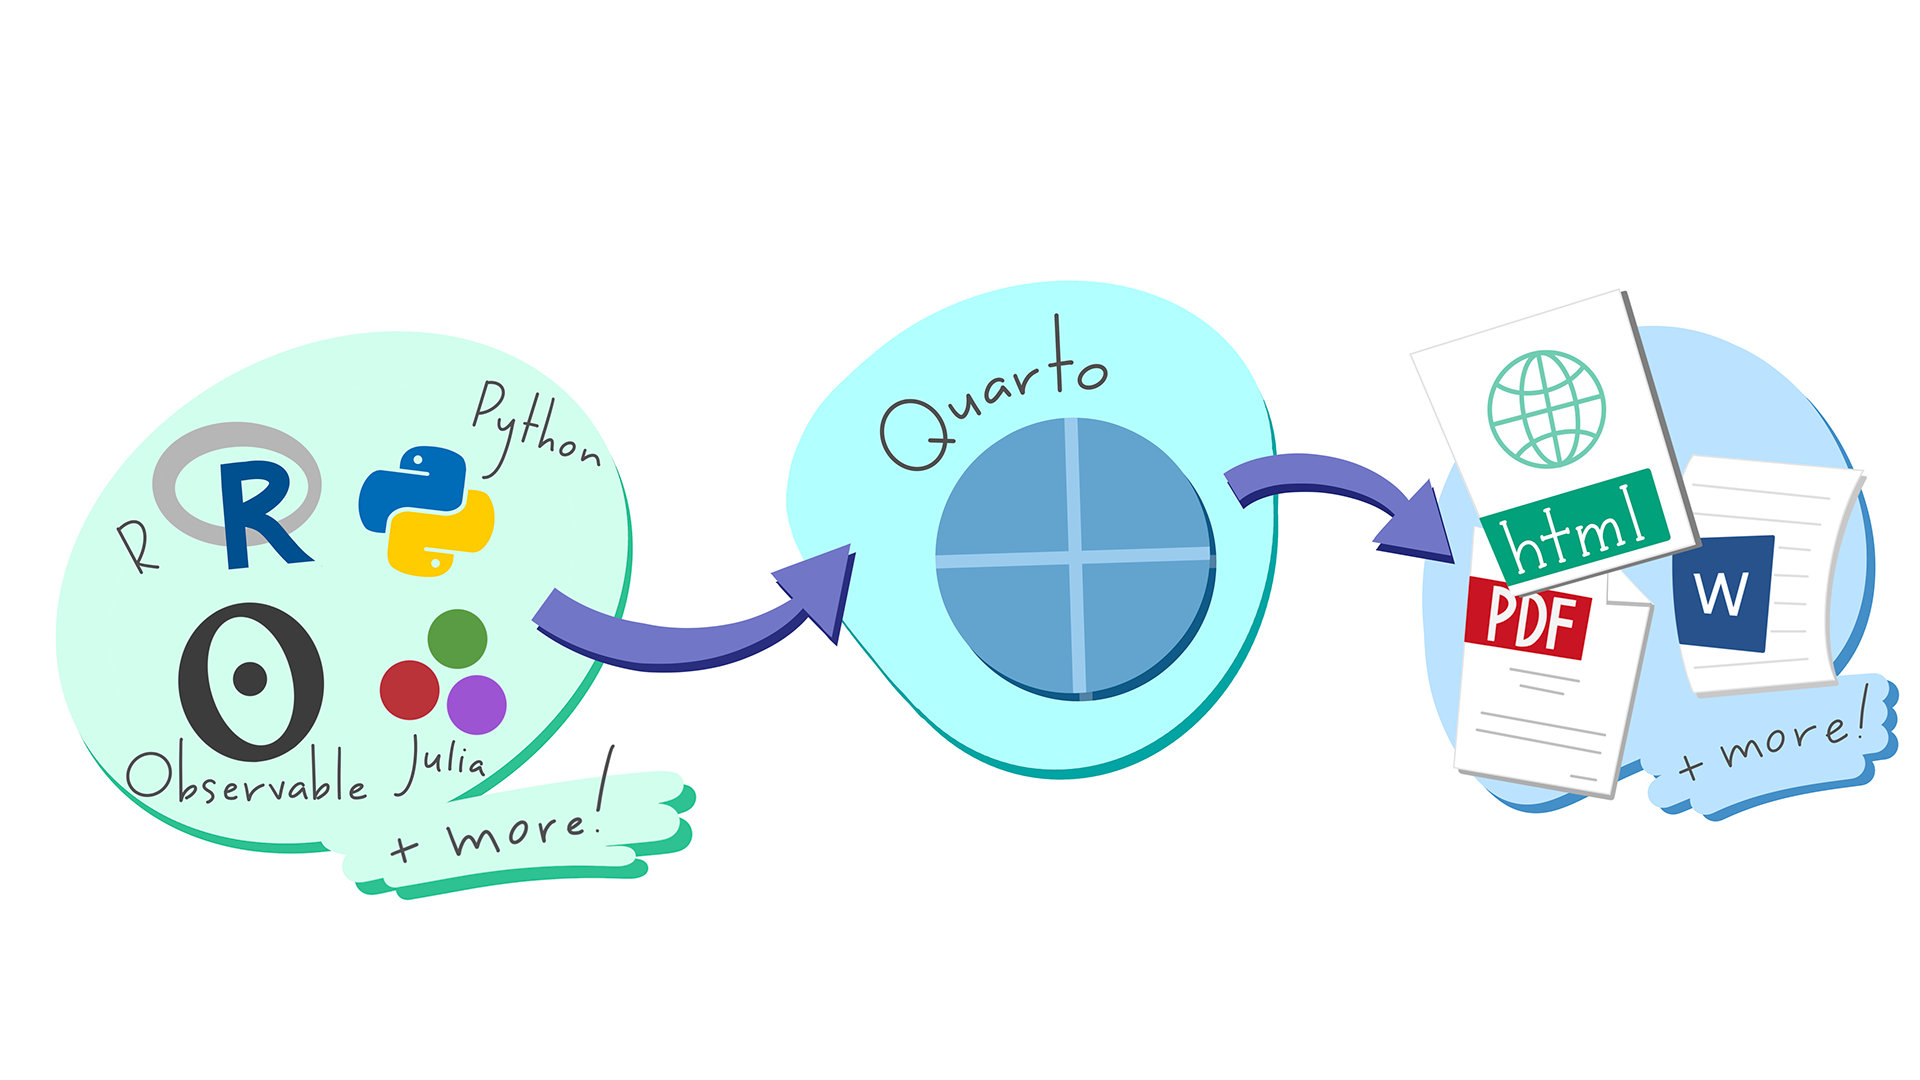
\includegraphics[keepaspectratio]{indexpdf_files/mediabag/quarto-illustration.png}}

}

\caption{\label{fig-logo}Logo de Quarto}

\end{figure}%

\subsection{Imagenes desde R}\label{imagenes-desde-r}

\subsubsection{Plot}\label{plot}

\begin{Shaded}
\begin{Highlighting}[]
\CommentTok{\# Filtrar los datos para Chile y Argentina}
\NormalTok{datos\_filtrados }\OtherTok{\textless{}{-}}\NormalTok{ gapminder }\SpecialCharTok{\%\textgreater{}\%}
  \FunctionTok{filter}\NormalTok{(country }\SpecialCharTok{\%in\%} \FunctionTok{c}\NormalTok{(}\StringTok{"Chile"}\NormalTok{, }\StringTok{"Argentina"}\NormalTok{))}

\CommentTok{\# Definir el rango de años y la esperanza de vida para el eje Y}
\NormalTok{years }\OtherTok{\textless{}{-}} \FunctionTok{unique}\NormalTok{(datos\_filtrados}\SpecialCharTok{$}\NormalTok{year)}
\NormalTok{ylim }\OtherTok{\textless{}{-}} \FunctionTok{range}\NormalTok{(datos\_filtrados}\SpecialCharTok{$}\NormalTok{lifeExp)}

\CommentTok{\# Crear el gráfico vacío}
\FunctionTok{plot}\NormalTok{(}\ConstantTok{NULL}\NormalTok{, }\AttributeTok{xlim =} \FunctionTok{range}\NormalTok{(years), }\AttributeTok{ylim =}\NormalTok{ ylim,}
     \AttributeTok{xlab =} \StringTok{"Año"}\NormalTok{, }\AttributeTok{ylab =} \StringTok{"Esperanza de Vida (años)"}\NormalTok{,}
     \AttributeTok{main =} \StringTok{"Evolución de la Esperanza de Vida en Chile y Argentina"}\NormalTok{)}

\CommentTok{\# Añadir líneas para cada país}
\NormalTok{countries }\OtherTok{\textless{}{-}} \FunctionTok{c}\NormalTok{(}\StringTok{"Chile"}\NormalTok{, }\StringTok{"Argentina"}\NormalTok{)}
\NormalTok{colors }\OtherTok{\textless{}{-}} \FunctionTok{c}\NormalTok{(}\StringTok{"blue"}\NormalTok{, }\StringTok{"red"}\NormalTok{)}

\ControlFlowTok{for}\NormalTok{ (i }\ControlFlowTok{in} \DecValTok{1}\SpecialCharTok{:}\DecValTok{2}\NormalTok{) \{}
\NormalTok{  country\_data }\OtherTok{\textless{}{-}}\NormalTok{ datos\_filtrados }\SpecialCharTok{\%\textgreater{}\%} \FunctionTok{filter}\NormalTok{(country }\SpecialCharTok{==}\NormalTok{ countries[i])}
  \FunctionTok{lines}\NormalTok{(country\_data}\SpecialCharTok{$}\NormalTok{year, country\_data}\SpecialCharTok{$}\NormalTok{lifeExp, }\AttributeTok{type =} \StringTok{"o"}\NormalTok{, }\AttributeTok{col =}\NormalTok{ colors[i], }\AttributeTok{pch =} \DecValTok{16}\NormalTok{)}
\NormalTok{\}}

\CommentTok{\# Añadir una leyenda}
\FunctionTok{legend}\NormalTok{(}\StringTok{"bottomright"}\NormalTok{, }\AttributeTok{legend =}\NormalTok{ countries, }\AttributeTok{col =}\NormalTok{ colors, }\AttributeTok{pch =} \DecValTok{16}\NormalTok{, }\AttributeTok{lty =} \DecValTok{1}\NormalTok{)}
\end{Highlighting}
\end{Shaded}

\begin{figure}[H]

\centering{

\pandocbounded{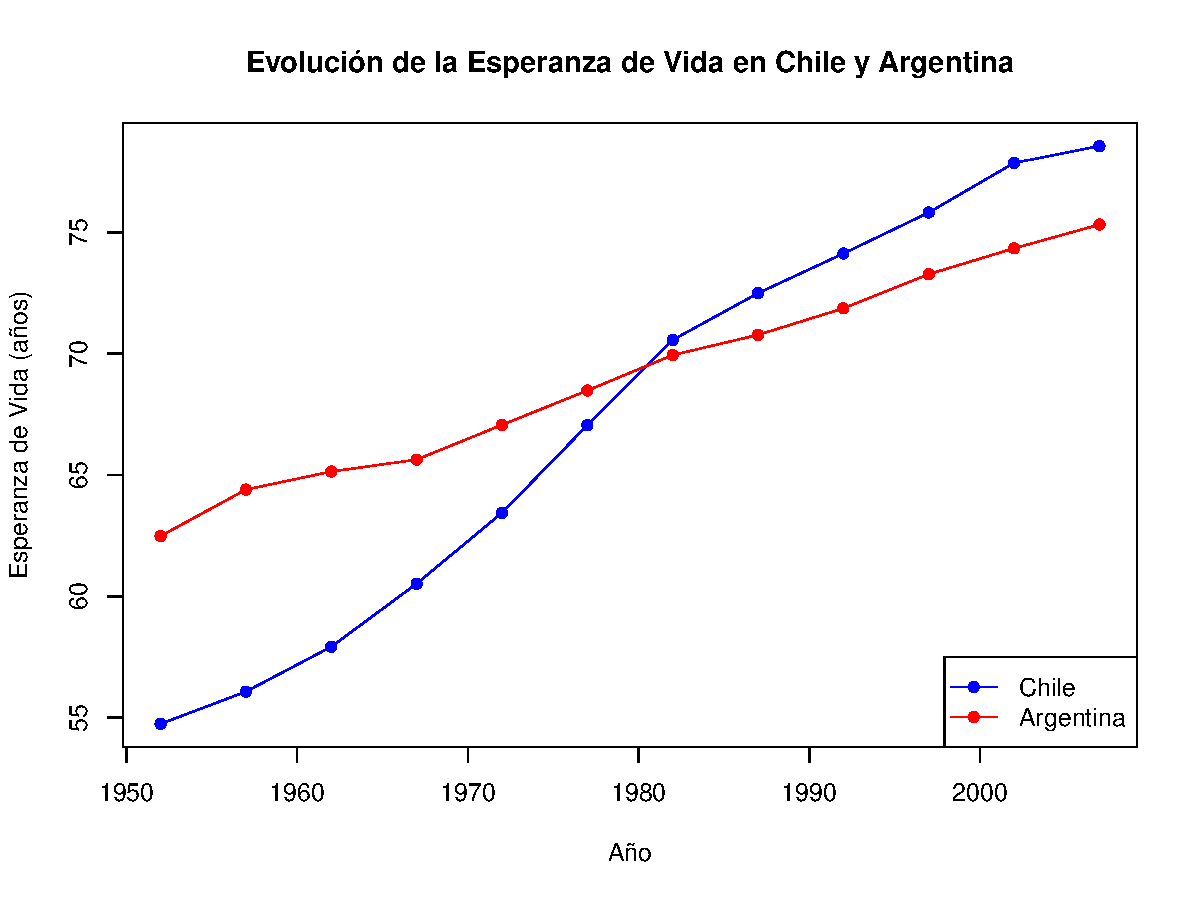
\includegraphics[keepaspectratio]{indexpdf_files/figure-pdf/fig-plot-1.pdf}}

}

\caption{\label{fig-plot}Gráfico de líneas en plot}

\end{figure}%

\subsubsection{Ggplot}\label{ggplot}

\begin{Shaded}
\begin{Highlighting}[]
\CommentTok{\# Crear el gráfico de líneas}
\FunctionTok{ggplot}\NormalTok{(datos\_filtrados, }\FunctionTok{aes}\NormalTok{(}\AttributeTok{x =}\NormalTok{ year, }\AttributeTok{y =}\NormalTok{ lifeExp, }\AttributeTok{color =}\NormalTok{ country)) }\SpecialCharTok{+}
  \FunctionTok{geom\_line}\NormalTok{(}\AttributeTok{size =} \DecValTok{1}\NormalTok{) }\SpecialCharTok{+}
  \FunctionTok{labs}\NormalTok{(}
    \AttributeTok{title =} \StringTok{"Evolución de la Esperanza de Vida en Chile y Argentina"}\NormalTok{,}
    \AttributeTok{x =} \StringTok{"Año"}\NormalTok{,}
    \AttributeTok{y =} \StringTok{"Esperanza de Vida (años)"}\NormalTok{,}
    \AttributeTok{color =} \StringTok{"País"}
\NormalTok{  ) }\SpecialCharTok{+}
  \FunctionTok{theme\_minimal}\NormalTok{()}
\end{Highlighting}
\end{Shaded}

\begin{figure}[H]

\centering{

\pandocbounded{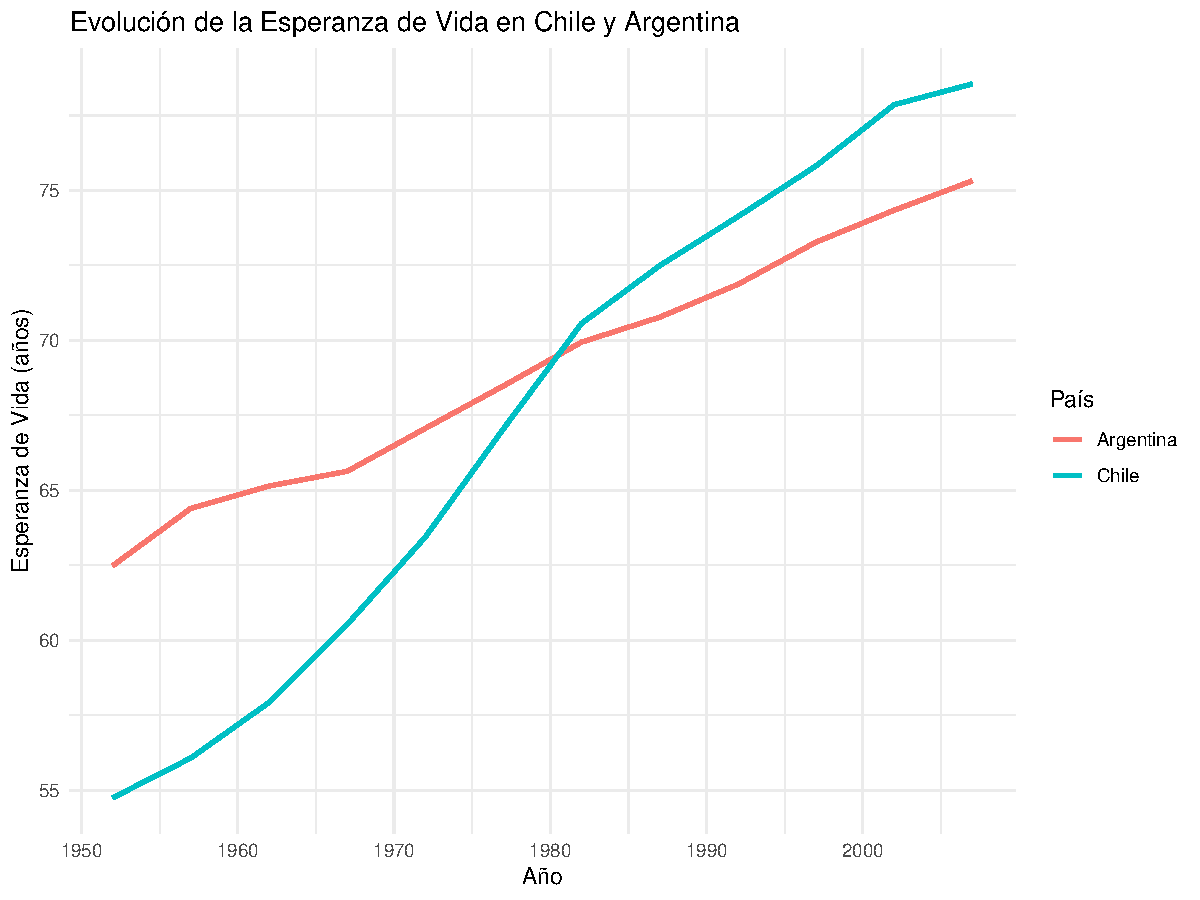
\includegraphics[keepaspectratio]{indexpdf_files/figure-pdf/fig-ggplot-1.pdf}}

}

\caption{\label{fig-ggplot}Gráfico de líneas en ggplot}

\end{figure}%

\subsubsection{Ggplot y LaTeX}\label{ggplot-y-latex}

\begin{Shaded}
\begin{Highlighting}[]
\CommentTok{\#Distribucion Normal}
\NormalTok{x }\OtherTok{\textless{}{-}} \FunctionTok{seq}\NormalTok{(}\AttributeTok{from =} \SpecialCharTok{{-}}\DecValTok{5}\NormalTok{, }\AttributeTok{to =} \DecValTok{5}\NormalTok{, }\AttributeTok{by =} \FloatTok{0.01}\NormalTok{)}
\NormalTok{norm\_dat }\OtherTok{\textless{}{-}} \FunctionTok{data.frame}\NormalTok{(x, }\AttributeTok{pdf =} \FunctionTok{dnorm}\NormalTok{(x,}\DecValTok{0}\NormalTok{,}\DecValTok{1}\NormalTok{))}
\NormalTok{quant }\OtherTok{\textless{}{-}} \FunctionTok{c}\NormalTok{(}\SpecialCharTok{{-}}\ConstantTok{Inf}\NormalTok{, }\SpecialCharTok{{-}}\FloatTok{1.96}\NormalTok{, }\FloatTok{1.96}\NormalTok{, }\ConstantTok{Inf}\NormalTok{)}
\NormalTok{norm\_dat}\SpecialCharTok{$}\NormalTok{quant }\OtherTok{\textless{}{-}} \FunctionTok{factor}\NormalTok{(}\FunctionTok{findInterval}\NormalTok{(norm\_dat}\SpecialCharTok{$}\NormalTok{x,quant))}

\CommentTok{\#grafico de funcion de densidad de probabilidades de la normal}
\FunctionTok{ggplot}\NormalTok{(norm\_dat, }\FunctionTok{aes}\NormalTok{(x,pdf)) }\SpecialCharTok{+} \FunctionTok{geom\_line}\NormalTok{()}\SpecialCharTok{+}  \FunctionTok{geom\_ribbon}\NormalTok{(}\FunctionTok{aes}\NormalTok{(}\AttributeTok{ymin=}\DecValTok{0}\NormalTok{, }\AttributeTok{ymax=}\NormalTok{pdf, }\AttributeTok{fill=}\NormalTok{quant), }\AttributeTok{alpha=}\FloatTok{0.5}\NormalTok{)}\SpecialCharTok{+}
  \FunctionTok{scale\_x\_continuous}\NormalTok{(}\AttributeTok{breaks=}\FunctionTok{seq}\NormalTok{(}\AttributeTok{from =} \SpecialCharTok{{-}}\DecValTok{5}\NormalTok{, }\AttributeTok{to =} \DecValTok{5}\NormalTok{, }\AttributeTok{by =} \DecValTok{1}\NormalTok{), }\AttributeTok{expand =} \FunctionTok{c}\NormalTok{(}\DecValTok{0}\NormalTok{, }\DecValTok{0}\NormalTok{))}\SpecialCharTok{+}
  \FunctionTok{scale\_y\_continuous}\NormalTok{(}\AttributeTok{limits =} \FunctionTok{c}\NormalTok{(}\DecValTok{0}\NormalTok{,}\FloatTok{0.45}\NormalTok{), }\AttributeTok{expand =} \FunctionTok{c}\NormalTok{(}\DecValTok{0}\NormalTok{, }\DecValTok{0}\NormalTok{))}\SpecialCharTok{+}
  \FunctionTok{geom\_vline}\NormalTok{(}\AttributeTok{xintercept=}\NormalTok{(}\FloatTok{1.96}\NormalTok{), }\AttributeTok{size=}\DecValTok{1}\NormalTok{, }\AttributeTok{color=}\StringTok{"red"}\NormalTok{)}\SpecialCharTok{+}
  \FunctionTok{geom\_vline}\NormalTok{(}\AttributeTok{xintercept=}\NormalTok{(}\SpecialCharTok{{-}}\FloatTok{1.96}\NormalTok{), }\AttributeTok{size=}\DecValTok{1}\NormalTok{, }\AttributeTok{color=}\StringTok{"red"}\NormalTok{)}\SpecialCharTok{+}
  \FunctionTok{scale\_fill\_manual}\NormalTok{(}\AttributeTok{values =} \FunctionTok{c}\NormalTok{(}\StringTok{"red"}\NormalTok{,}\StringTok{"grey"}\NormalTok{,}\StringTok{"red"}\NormalTok{))}\SpecialCharTok{+}
  \FunctionTok{theme\_bw}\NormalTok{() }\SpecialCharTok{+} \FunctionTok{theme}\NormalTok{(}\AttributeTok{legend.position =} \StringTok{"none"}\NormalTok{)}\SpecialCharTok{+}
  \FunctionTok{ylab}\NormalTok{(latex2exp}\SpecialCharTok{::}\FunctionTok{TeX}\NormalTok{(}\StringTok{"$ = }\SpecialCharTok{\textbackslash{}\textbackslash{}}\StringTok{frac\{1\}\{}\SpecialCharTok{\textbackslash{}\textbackslash{}}\StringTok{sigma}\SpecialCharTok{\textbackslash{}\textbackslash{}}\StringTok{sqrt\{2}\SpecialCharTok{\textbackslash{}\textbackslash{}}\StringTok{pi\}\}}\SpecialCharTok{\textbackslash{}\textbackslash{}}\StringTok{exp}\SpecialCharTok{\textbackslash{}\textbackslash{}}\StringTok{left({-}}\SpecialCharTok{\textbackslash{}\textbackslash{}}\StringTok{frac\{1\}\{2\}}\SpecialCharTok{\textbackslash{}\textbackslash{}}\StringTok{left(}\SpecialCharTok{\textbackslash{}\textbackslash{}}\StringTok{frac\{x{-}}\SpecialCharTok{\textbackslash{}\textbackslash{}}\StringTok{mu\}\{}\SpecialCharTok{\textbackslash{}\textbackslash{}}\StringTok{sigma\}}\SpecialCharTok{\textbackslash{}\textbackslash{}}\StringTok{right)\^{}\{}\SpecialCharTok{\textbackslash{}\textbackslash{}}\StringTok{2\}}\SpecialCharTok{\textbackslash{}\textbackslash{}}\StringTok{,}\SpecialCharTok{\textbackslash{}\textbackslash{}}\StringTok{right)$"}\NormalTok{))}\SpecialCharTok{+}
  \FunctionTok{xlab}\NormalTok{(latex2exp}\SpecialCharTok{::}\FunctionTok{TeX}\NormalTok{(}\StringTok{"$}\SpecialCharTok{\textbackslash{}\textbackslash{}}\StringTok{z\_0$"}\NormalTok{ ))}\SpecialCharTok{+}
  \FunctionTok{annotate}\NormalTok{(}\AttributeTok{geom =} \StringTok{"text"}\NormalTok{,}
           \AttributeTok{label =} \StringTok{"1,96"}\NormalTok{,}
           \AttributeTok{x =} \FloatTok{1.96}\NormalTok{,}
           \AttributeTok{y =} \FloatTok{0.3}\NormalTok{,}
           \AttributeTok{angle =} \DecValTok{90}\NormalTok{, }
           \AttributeTok{vjust =} \SpecialCharTok{{-}}\DecValTok{1}\NormalTok{,}
           \AttributeTok{colour =} \StringTok{"red"}\NormalTok{,}
           \AttributeTok{size =} \DecValTok{8}\NormalTok{)}\SpecialCharTok{+}
  \FunctionTok{annotate}\NormalTok{(}\AttributeTok{geom =} \StringTok{"text"}\NormalTok{,}
           \AttributeTok{label =} \StringTok{"{-}1,96"}\NormalTok{,}
           \AttributeTok{x =} \SpecialCharTok{{-}}\FloatTok{1.96}\NormalTok{,}
           \AttributeTok{y =} \FloatTok{0.3}\NormalTok{,}
           \AttributeTok{angle =} \DecValTok{90}\NormalTok{, }
           \AttributeTok{vjust =} \SpecialCharTok{{-}}\DecValTok{1}\NormalTok{,}
           \AttributeTok{colour =} \StringTok{"red"}\NormalTok{,}
           \AttributeTok{size =} \DecValTok{8}\NormalTok{)}
\end{Highlighting}
\end{Shaded}

\begin{figure}[H]

\centering{

\pandocbounded{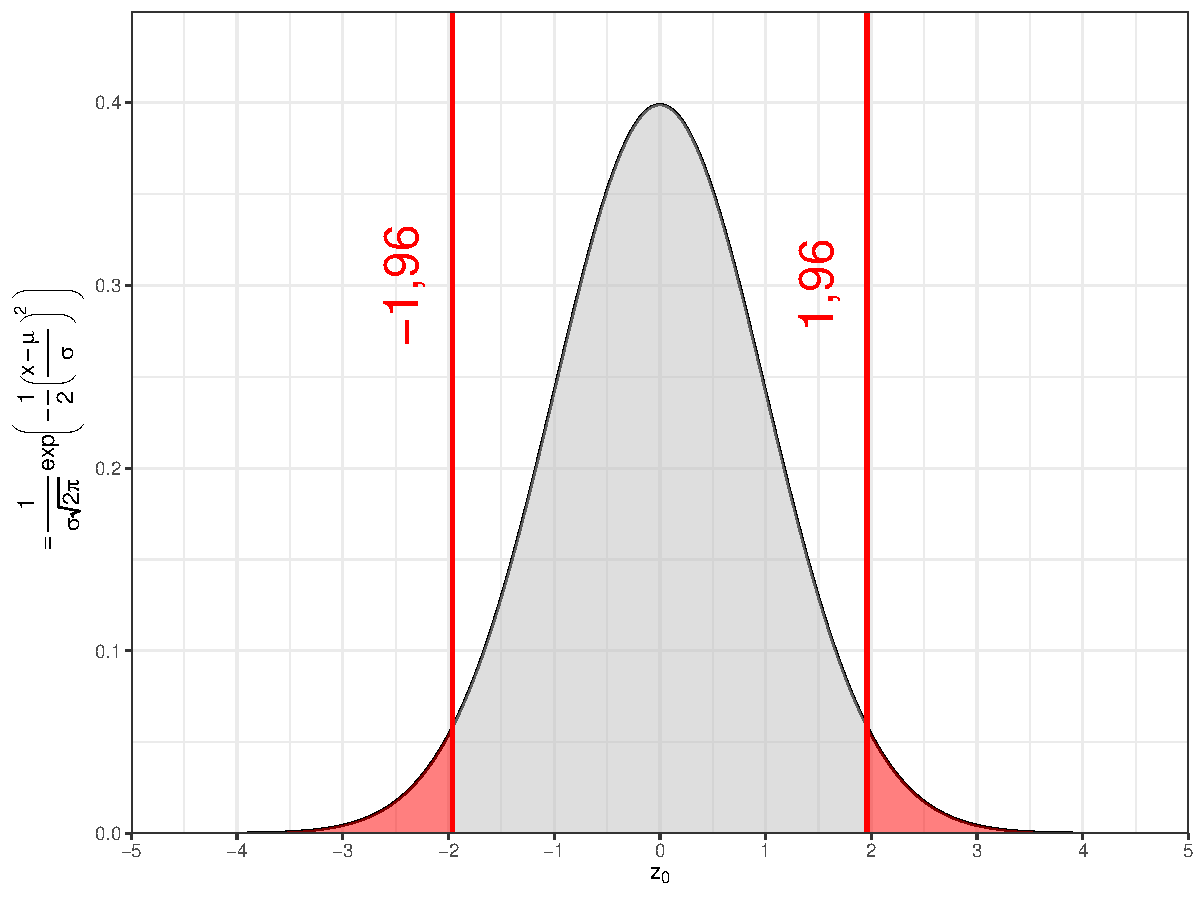
\includegraphics[keepaspectratio]{indexpdf_files/figure-pdf/fig-ggplot-tex-1.pdf}}

}

\caption{\label{fig-ggplot-tex}Distribución Normal}

\end{figure}%

\subsubsection{Mapas con maps}\label{mapas-con-maps}

\begin{Shaded}
\begin{Highlighting}[]
\CommentTok{\# Cargar el mapa de un país o región (ejemplo: Chile)}
\NormalTok{map\_data }\OtherTok{\textless{}{-}} \FunctionTok{map\_data}\NormalTok{(}\StringTok{"world"}\NormalTok{, }\AttributeTok{region =} \StringTok{"Chile"}\NormalTok{)}

\CommentTok{\# Crear el gráfico del mapa}
\FunctionTok{ggplot}\NormalTok{(}\AttributeTok{data =}\NormalTok{ map\_data) }\SpecialCharTok{+}
  \FunctionTok{geom\_polygon}\NormalTok{(}\FunctionTok{aes}\NormalTok{(}\AttributeTok{x =}\NormalTok{ long, }\AttributeTok{y =}\NormalTok{ lat, }\AttributeTok{group =}\NormalTok{ group), }\AttributeTok{fill =} \StringTok{"lightblue"}\NormalTok{, }\AttributeTok{color =} \StringTok{"black"}\NormalTok{) }\SpecialCharTok{+}
  \FunctionTok{coord\_fixed}\NormalTok{(}\FloatTok{1.3}\NormalTok{) }\SpecialCharTok{+}  \CommentTok{\# Mantiene las proporciones}
  \FunctionTok{labs}\NormalTok{(}\AttributeTok{title =} \StringTok{"Mapa de Chile"}\NormalTok{) }\SpecialCharTok{+}
  \FunctionTok{theme\_minimal}\NormalTok{()}
\end{Highlighting}
\end{Shaded}

\begin{figure}[H]

\centering{

\pandocbounded{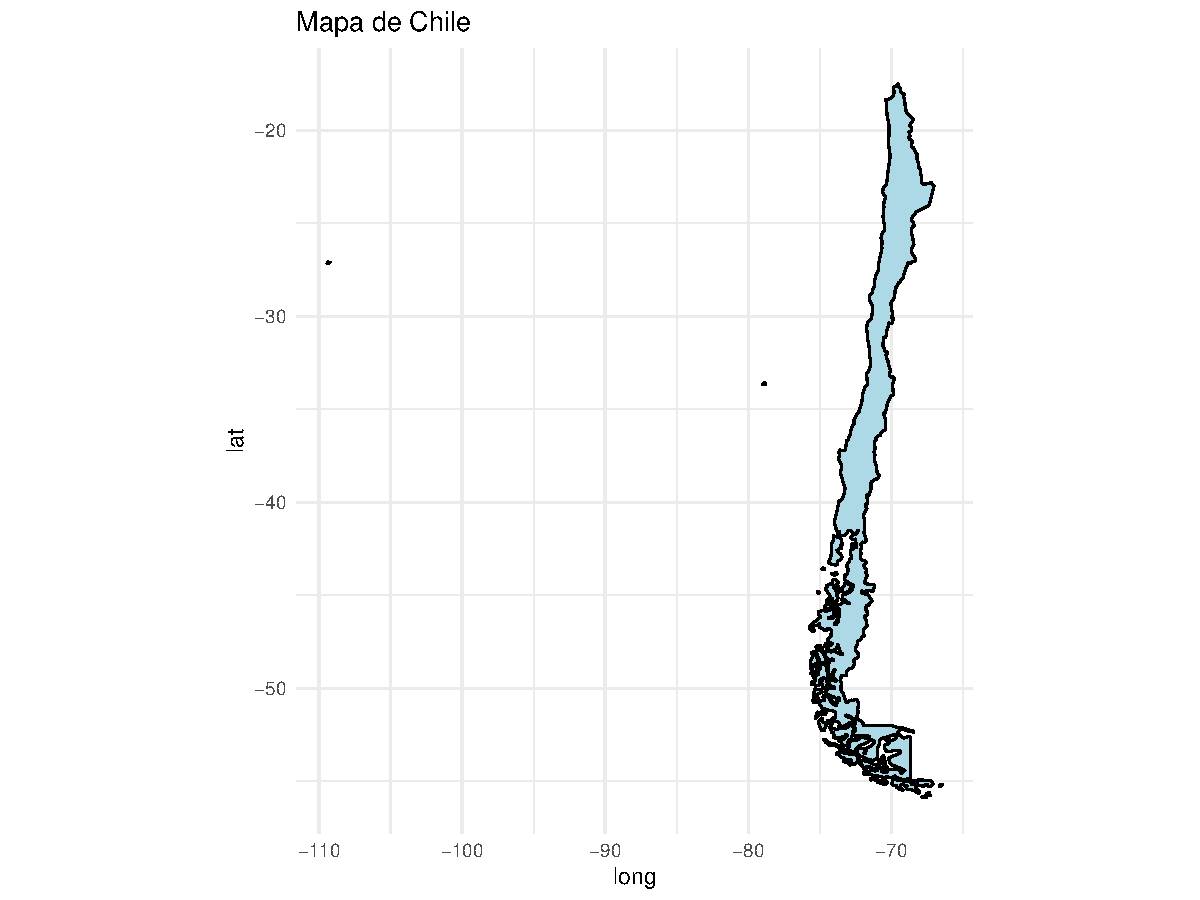
\includegraphics[keepaspectratio]{indexpdf_files/figure-pdf/fig-maps-1.pdf}}

}

\caption{\label{fig-maps}Chile}

\end{figure}%

\subsubsection{Mapas con sf}\label{mapas-con-sf}

\begin{Shaded}
\begin{Highlighting}[]
\CommentTok{\# Cargar datos de ejemplo del paquete sf}
\NormalTok{world }\OtherTok{\textless{}{-}} \FunctionTok{st\_read}\NormalTok{(}\FunctionTok{system.file}\NormalTok{(}\StringTok{"shape/nc.shp"}\NormalTok{, }\AttributeTok{package =} \StringTok{"sf"}\NormalTok{), }\AttributeTok{quiet =} \ConstantTok{TRUE}\NormalTok{)}

\CommentTok{\# Graficar el mapa}
\FunctionTok{ggplot}\NormalTok{(}\AttributeTok{data =}\NormalTok{ world) }\SpecialCharTok{+}
  \FunctionTok{geom\_sf}\NormalTok{(}\AttributeTok{fill =} \StringTok{"lightblue"}\NormalTok{, }\AttributeTok{color =} \StringTok{"black"}\NormalTok{) }\SpecialCharTok{+}
  \FunctionTok{labs}\NormalTok{(}\AttributeTok{title =} \StringTok{"Mapa de Ejemplo (Datos de sf)"}\NormalTok{) }\SpecialCharTok{+}
  \FunctionTok{theme\_minimal}\NormalTok{()}
\end{Highlighting}
\end{Shaded}

\begin{figure}[H]

\centering{

\pandocbounded{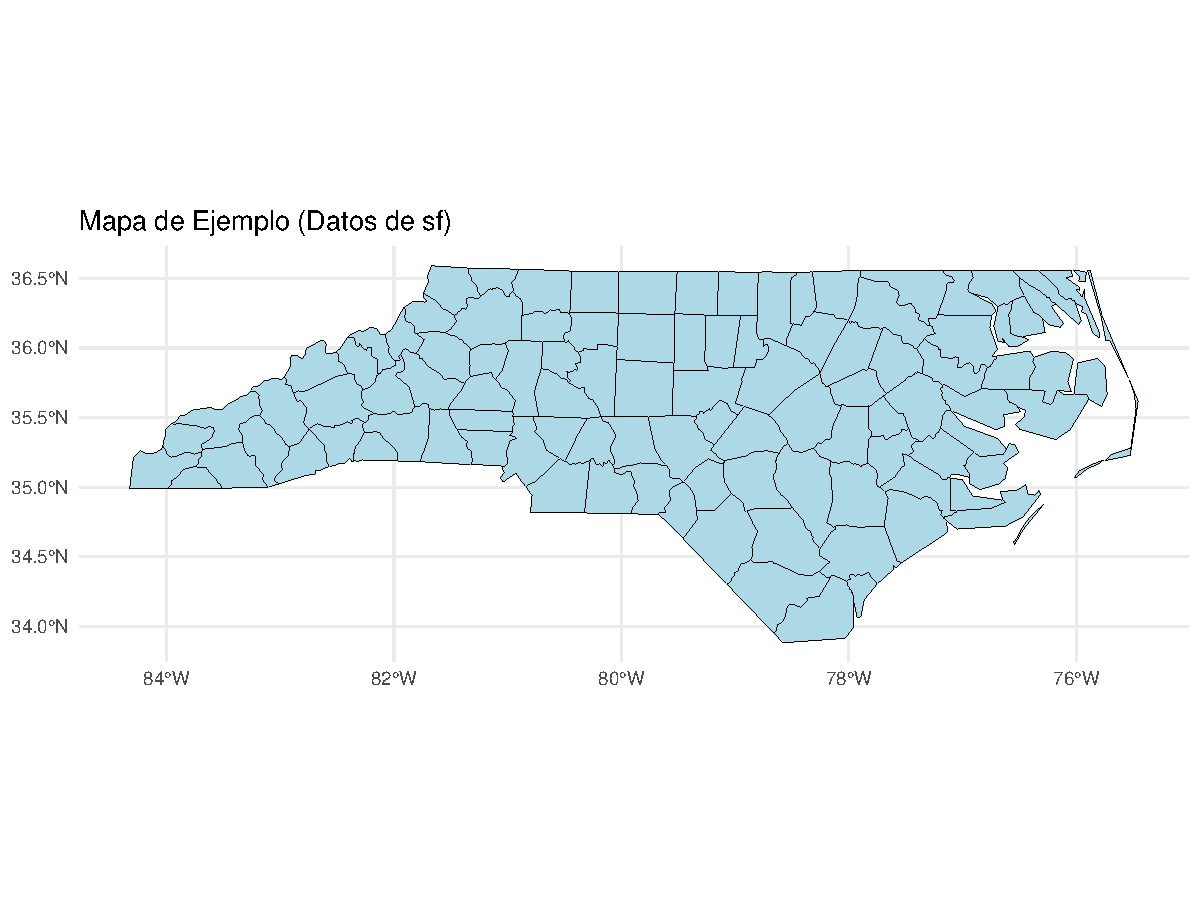
\includegraphics[keepaspectratio]{indexpdf_files/figure-pdf/fig-sf-1.pdf}}

}

\caption{\label{fig-sf}Carolina del Norte (Estados Unidos).}

\end{figure}%

\begin{Shaded}
\begin{Highlighting}[]
\CommentTok{\# Crear un mapa estático}
\FunctionTok{data}\NormalTok{(}\StringTok{"World"}\NormalTok{, }\AttributeTok{package =} \StringTok{"tmap"}\NormalTok{)}

\CommentTok{\# Cambiar a modo de mapa estático}
\FunctionTok{tmap\_mode}\NormalTok{(}\StringTok{"plot"}\NormalTok{)}

\CommentTok{\# Crear el mapa}
\NormalTok{map }\OtherTok{\textless{}{-}} \FunctionTok{tm\_shape}\NormalTok{(World) }\SpecialCharTok{+}
  \FunctionTok{tm\_polygons}\NormalTok{(}\StringTok{"HPI"}\NormalTok{, }\AttributeTok{title =} \StringTok{"Índice de Planeta Feliz (HPI)"}\NormalTok{) }\SpecialCharTok{+}
  \FunctionTok{tm\_layout}\NormalTok{(}\AttributeTok{title =} \StringTok{"Mapa Mundial"}\NormalTok{)}
\NormalTok{map}
\end{Highlighting}
\end{Shaded}

\begin{figure}[H]

\centering{

\pandocbounded{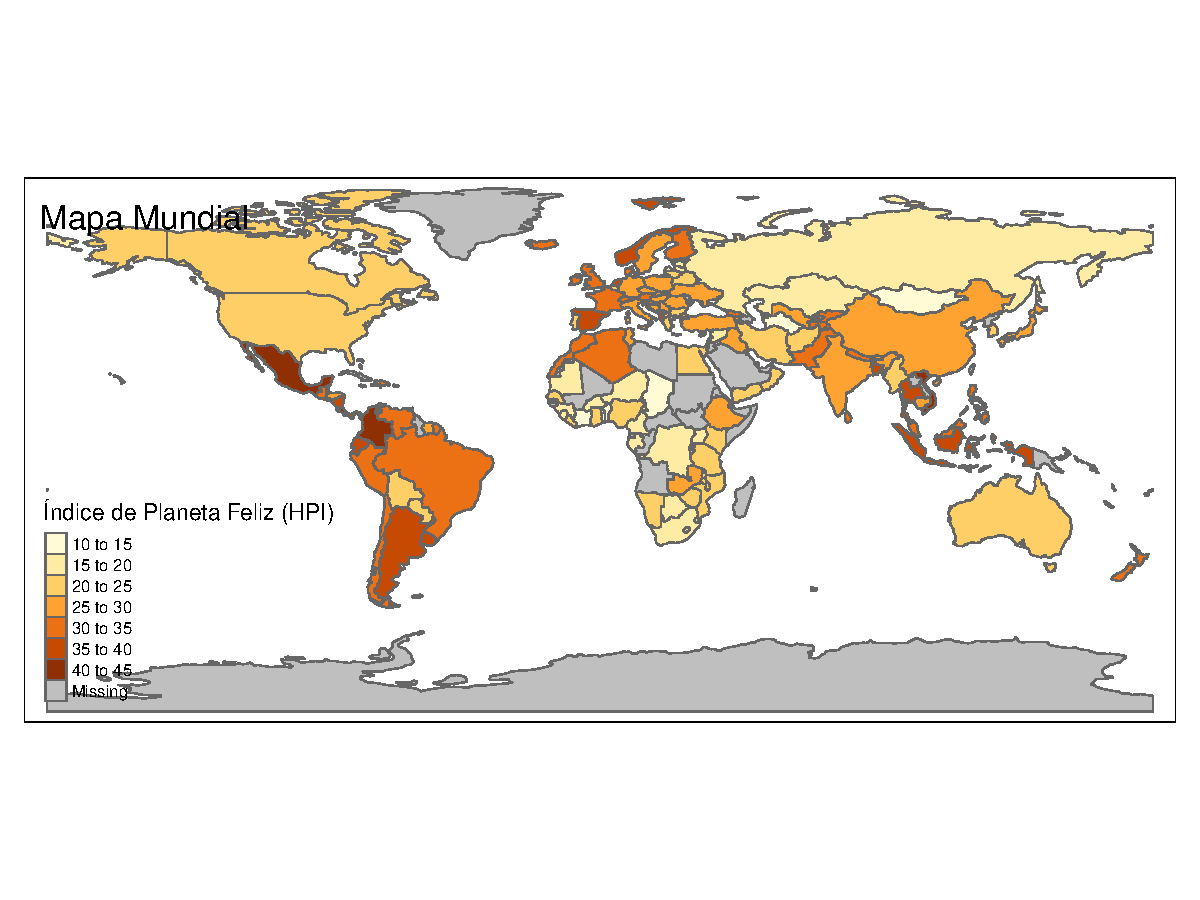
\includegraphics[keepaspectratio]{indexpdf_files/figure-pdf/fig-tmap-1.pdf}}

}

\caption{\label{fig-tmap}Mapa Mundial.}

\end{figure}%

\begin{Shaded}
\begin{Highlighting}[]
\CommentTok{\# pip install seaborn matplotlib scikit{-}learn pandas plotly}
\end{Highlighting}
\end{Shaded}

\begin{Shaded}
\begin{Highlighting}[]
\ImportTok{import}\NormalTok{ matplotlib.pyplot }\ImportTok{as}\NormalTok{ plt}
\ImportTok{import}\NormalTok{ numpy }\ImportTok{as}\NormalTok{ np}

\CommentTok{\# Crear datos}
\NormalTok{x }\OperatorTok{=}\NormalTok{ np.linspace(}\DecValTok{0}\NormalTok{, }\DecValTok{10}\NormalTok{, }\DecValTok{100}\NormalTok{)}
\NormalTok{y }\OperatorTok{=}\NormalTok{ np.sin(x)}

\CommentTok{\# Generar la figura}
\NormalTok{plt.figure(figsize}\OperatorTok{=}\NormalTok{(}\DecValTok{8}\NormalTok{, }\DecValTok{6}\NormalTok{))}
\NormalTok{plt.plot(x, y, label}\OperatorTok{=}\StringTok{"Seno(x)"}\NormalTok{, color}\OperatorTok{=}\StringTok{"blue"}\NormalTok{)}
\NormalTok{plt.title(}\StringTok{"Gráfico generado con Python en Quarto"}\NormalTok{)}
\NormalTok{plt.xlabel(}\StringTok{"Eje X"}\NormalTok{)}
\NormalTok{plt.ylabel(}\StringTok{"Eje Y"}\NormalTok{)}
\NormalTok{plt.legend()}
\NormalTok{plt.grid(}\VariableTok{True}\NormalTok{)}

\CommentTok{\# Mostrar la figura}
\NormalTok{plt.show()}
\end{Highlighting}
\end{Shaded}

\begin{figure}[H]

\centering{

\pandocbounded{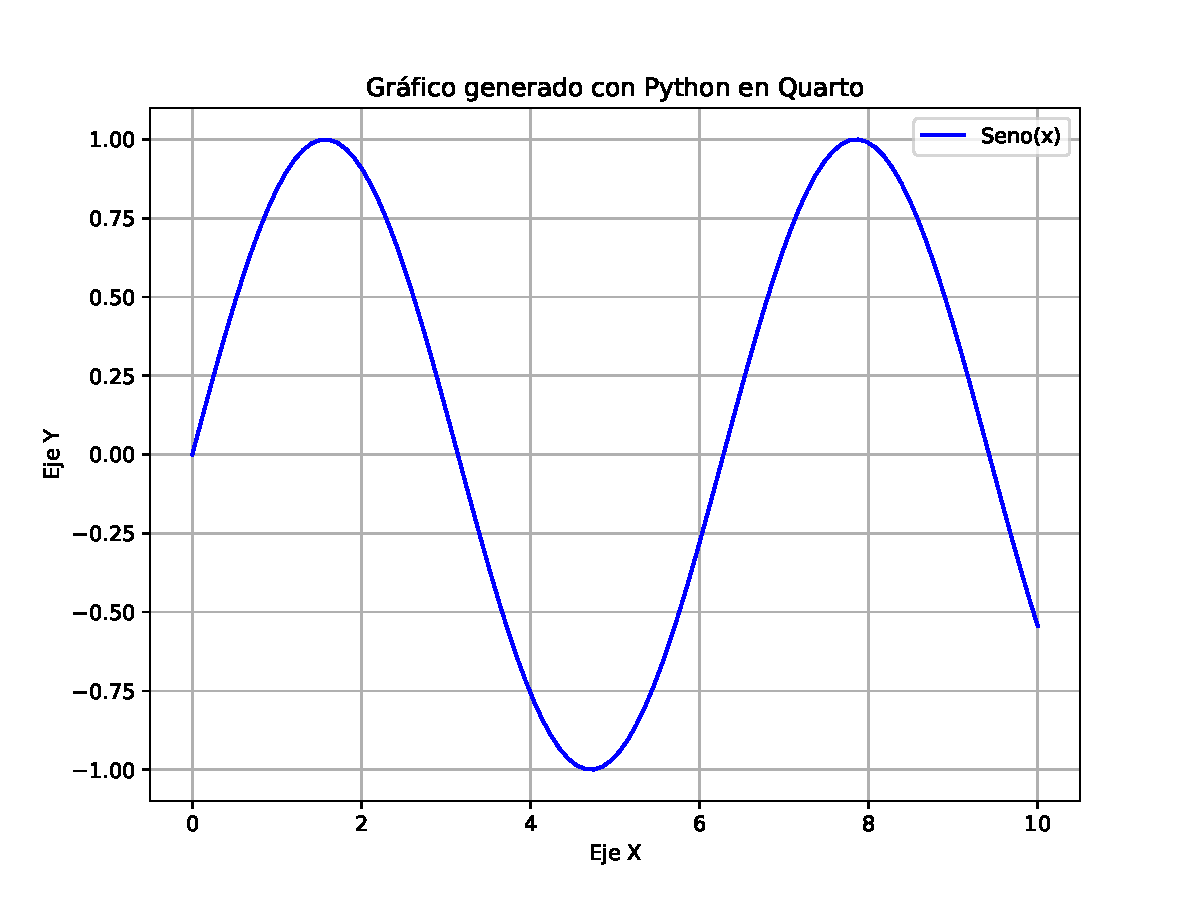
\includegraphics[keepaspectratio]{indexpdf_files/figure-pdf/fig-python-1.pdf}}

}

\caption{\label{fig-python}Grafico Python 1}

\end{figure}%

\begin{Shaded}
\begin{Highlighting}[]
\ImportTok{import}\NormalTok{ seaborn }\ImportTok{as}\NormalTok{ sns}
\ImportTok{import}\NormalTok{ matplotlib.pyplot }\ImportTok{as}\NormalTok{ plt}
\ImportTok{from}\NormalTok{ sklearn.datasets }\ImportTok{import}\NormalTok{ load\_iris}
\ImportTok{import}\NormalTok{ pandas }\ImportTok{as}\NormalTok{ pd}

\CommentTok{\# Cargar el dataset de ejemplo}
\NormalTok{data }\OperatorTok{=}\NormalTok{ load\_iris()}
\NormalTok{df }\OperatorTok{=}\NormalTok{ pd.DataFrame(data.data, columns}\OperatorTok{=}\NormalTok{data.feature\_names)}
\NormalTok{df[}\StringTok{\textquotesingle{}species\textquotesingle{}}\NormalTok{] }\OperatorTok{=}\NormalTok{ data.target}

\CommentTok{\# Crear un gráfico con seaborn}
\NormalTok{sns.}\BuiltInTok{set}\NormalTok{(style}\OperatorTok{=}\StringTok{"whitegrid"}\NormalTok{)}
\NormalTok{plt.figure(figsize}\OperatorTok{=}\NormalTok{(}\DecValTok{10}\NormalTok{, }\DecValTok{6}\NormalTok{))}
\NormalTok{sns.boxplot(data}\OperatorTok{=}\NormalTok{df, x}\OperatorTok{=}\StringTok{\textquotesingle{}species\textquotesingle{}}\NormalTok{, y}\OperatorTok{=}\StringTok{\textquotesingle{}sepal length (cm)\textquotesingle{}}\NormalTok{, palette}\OperatorTok{=}\StringTok{\textquotesingle{}viridis\textquotesingle{}}\NormalTok{)}

\CommentTok{\# Configurar el título}
\NormalTok{plt.title(}\StringTok{"Distribución de la longitud del sépalo por especie"}\NormalTok{, fontsize}\OperatorTok{=}\DecValTok{14}\NormalTok{)}
\NormalTok{plt.xlabel(}\StringTok{"Especie"}\NormalTok{, fontsize}\OperatorTok{=}\DecValTok{12}\NormalTok{)}
\NormalTok{plt.ylabel(}\StringTok{"Longitud del Sépalo (cm)"}\NormalTok{, fontsize}\OperatorTok{=}\DecValTok{12}\NormalTok{)}

\CommentTok{\# Mostrar la figura}
\NormalTok{plt.show()}
\end{Highlighting}
\end{Shaded}

\begin{figure}[H]

\centering{

\pandocbounded{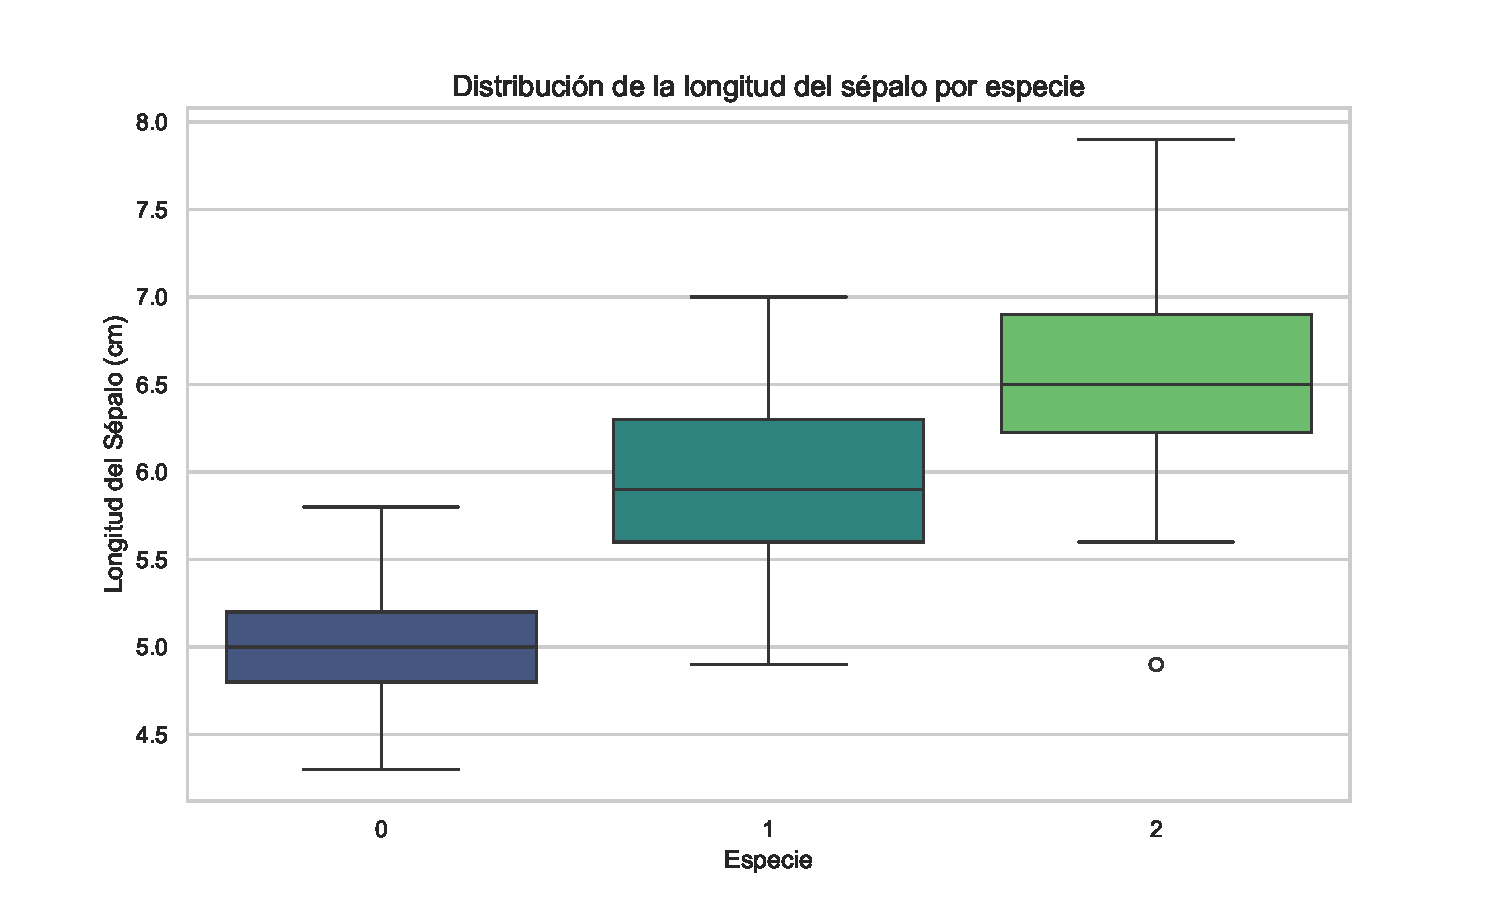
\includegraphics[keepaspectratio]{indexpdf_files/figure-pdf/fig-python2-3.pdf}}

}

\caption{\label{fig-python2}Grafico Python 2}

\end{figure}%

\subsubsection{Citar figuras en el
texto}\label{citar-figuras-en-el-texto}

La Figura~\ref{fig-plot}, Figura~\ref{fig-ggplot}, la
Figura~\ref{fig-sf} son\ldots{}

\section{Tablas}\label{tablas-1}

\subsection{Table1}\label{table1}

\begin{Shaded}
\begin{Highlighting}[]
\CommentTok{\# Filtrar datos de Gapminder para 2007}
\NormalTok{data\_gap }\OtherTok{\textless{}{-}}\NormalTok{ gapminder }\SpecialCharTok{\%\textgreater{}\%} \FunctionTok{filter}\NormalTok{(year }\SpecialCharTok{==} \DecValTok{2007}\NormalTok{)}

\CommentTok{\# Etiquetas descriptivas}
\FunctionTok{label}\NormalTok{(data\_gap}\SpecialCharTok{$}\NormalTok{lifeExp) }\OtherTok{\textless{}{-}} \StringTok{"Esperanza de Vida (años)"}
\FunctionTok{label}\NormalTok{(data\_gap}\SpecialCharTok{$}\NormalTok{gdpPercap) }\OtherTok{\textless{}{-}} \StringTok{"PIB per cápita (USD)"}
\FunctionTok{label}\NormalTok{(data\_gap}\SpecialCharTok{$}\NormalTok{continent) }\OtherTok{\textless{}{-}} \StringTok{"Continente"}
\FunctionTok{label}\NormalTok{(data\_gap}\SpecialCharTok{$}\NormalTok{pop) }\OtherTok{\textless{}{-}} \StringTok{"Población Total"}
\end{Highlighting}
\end{Shaded}

\begin{table}[!ht]
\captionsetup{position=top} % Asegura que el caption esté arriba
\caption{Resumen de Indicadores Sociodemográficos por Continente (2007)}
\centering
\rotatebox{0}{
\resizebox{\textwidth}{!}{

\begin{tabular}[t]{lllllll}
\toprule
  & Africa & Americas & Asia & Europe & Oceania & Overall\\
\midrule
 & (N=52) & (N=25) & (N=33) & (N=30) & (N=2) & (N=142)\\
\addlinespace[0.3em]
\multicolumn{7}{l}{\textbf{Esperanza de Vida (años)}}\\
\hspace{1em}Mean (SD) & 54.8 (9.63) & 73.6 (4.44) & 70.7 (7.96) & 77.6 (2.98) & 80.7 (0.729) & 67.0 (12.1)\\
\hspace{1em}Median [Min, Max] & 52.9 [39.6, 76.4] & 72.9 [60.9, 80.7] & 72.4 [43.8, 82.6] & 78.6 [71.8, 81.8] & 80.7 [80.2, 81.2] & 71.9 [39.6, 82.6]\\
\addlinespace[0.3em]
\multicolumn{7}{l}{\textbf{PIB per cápita (USD)}}\\
\hspace{1em}Mean (SD) & 3090 (3620) & 11000 (9710) & 12500 (14200) & 25100 (11800) & 29800 (6540) & 11700 (12900)\\
\hspace{1em}Median [Min, Max] & 1450 [278, 13200] & 8950 [1200, 43000] & 4470 [944, 47300] & 28100 [5940, 49400] & 29800 [25200, 34400] & 6120 [278, 49400]\\
\addlinespace[0.3em]
\multicolumn{7}{l}{\textbf{Población Total}}\\
\hspace{1em}Mean (SD) & 17900000 (24900000) & 36000000 (68800000) & 116000000 (290000000) & 19500000 (23600000) & 12300000 (11500000) & 44000000 (148000000)\\
\hspace{1em}Median [Min, Max] & 10100000 [200000, 135000000] & 9320000 [1060000, 301000000] & 24800000 [709000, 1320000000] & 9490000 [302000, 82400000] & 12300000 [4120000, 20400000] & 10500000 [200000, 1320000000]\\
\bottomrule
\end{tabular}


}
}
\end{table}

\href{https://cran.r-project.org/web/packages/table1/vignettes/table1-examples.html}{Opciones
table1}.

\newpage

\subsection{Kable}\label{kable}

\begin{Shaded}
\begin{Highlighting}[]
\CommentTok{\# Crear un resumen de datos por continente}
\NormalTok{tabla\_gap }\OtherTok{\textless{}{-}}\NormalTok{ data\_gap }\SpecialCharTok{\%\textgreater{}\%}
  \FunctionTok{group\_by}\NormalTok{(continent) }\SpecialCharTok{\%\textgreater{}\%}
  \FunctionTok{summarise}\NormalTok{(}
    \StringTok{\textasciigrave{}}\AttributeTok{Esperanza de Vida Promedio}\StringTok{\textasciigrave{}} \OtherTok{=} \FunctionTok{round}\NormalTok{(}\FunctionTok{mean}\NormalTok{(lifeExp), }\DecValTok{1}\NormalTok{),}
    \StringTok{\textasciigrave{}}\AttributeTok{PIB per cápita Promedio (USD)}\StringTok{\textasciigrave{}} \OtherTok{=} \FunctionTok{round}\NormalTok{(}\FunctionTok{mean}\NormalTok{(gdpPercap), }\DecValTok{2}\NormalTok{),}
    \StringTok{\textasciigrave{}}\AttributeTok{Población Total}\StringTok{\textasciigrave{}} \OtherTok{=} \FunctionTok{format}\NormalTok{(}\FunctionTok{sum}\NormalTok{(pop), }\AttributeTok{big.mark =} \StringTok{","}\NormalTok{)}
\NormalTok{  )}

\CommentTok{\# Crear tabla bien formateada para PDF}
\NormalTok{tabla\_gap }\SpecialCharTok{\%\textgreater{}\%}
  \FunctionTok{kbl}\NormalTok{(}\AttributeTok{caption =} \StringTok{"Resumen de Indicadores Sociodemográficos por Continente (2007)"}\NormalTok{,}
    \AttributeTok{booktabs =} \ConstantTok{TRUE}\NormalTok{) }\SpecialCharTok{\%\textgreater{}\%}
  \FunctionTok{kable\_styling}\NormalTok{(}
    \AttributeTok{latex\_options =} \FunctionTok{c}\NormalTok{(}\StringTok{"striped"}\NormalTok{, }\StringTok{"hold\_position"}\NormalTok{),}
    \AttributeTok{font\_size =} \DecValTok{10}
\NormalTok{  )}
\end{Highlighting}
\end{Shaded}

\begin{table}[!h]
\centering
\caption{Resumen de Indicadores Sociodemográficos por Continente (2007)}
\centering
\fontsize{10}{12}\selectfont
\begin{tabular}[t]{lrrl}
\toprule
continent & Esperanza de Vida Promedio & PIB per cápita Promedio (USD) & Población Total\\
\midrule
\cellcolor{gray!10}{Africa} & \cellcolor{gray!10}{54.8} & \cellcolor{gray!10}{3089.03} & \cellcolor{gray!10}{929,539,692}\\
Americas & 73.6 & 11003.03 & 898,871,184\\
\cellcolor{gray!10}{Asia} & \cellcolor{gray!10}{70.7} & \cellcolor{gray!10}{12473.03} & \cellcolor{gray!10}{3,811,953,827}\\
Europe & 77.6 & 25054.48 & 586,098,529\\
\cellcolor{gray!10}{Oceania} & \cellcolor{gray!10}{80.7} & \cellcolor{gray!10}{29810.19} & \cellcolor{gray!10}{24,549,947}\\
\bottomrule
\end{tabular}
\end{table}

\href{https://cran.r-project.org/web/packages/kableExtra/vignettes/awesome_table_in_html.html}{Opciones
kableExtra}.

\phantomsection\label{refs}
\begin{CSLReferences}{1}{0}
\bibitem[\citeproctext]{ref-chiang1984life}
1. Chiang, C. L. (1984). \emph{The Life Table and Its Applications}.
R.E. Krieger Publishing Company.
\url{https://books.google.cl/books?id=T_PrAAAAIAAJ}

\bibitem[\citeproctext]{ref-https:ux2fux2fdoi.orgux2f10.1002ux2fsim.4780100317}
2. Dobson, A. J., Kuulasmaa, K., Eberle, E., \& Scherer, J. (1991).
Confidence intervals for weighted sums of poisson parameters.
\emph{Statistics in Medicine}, \emph{10}(3), 457-462.
\url{https://doi.org//10.1002/sim.4780100317}

\bibitem[\citeproctext]{ref-worldbank_population_data}
3. World Bank. (2023). \emph{{World Bank Open Data: Female Population in
Chile}}.
\url{https://data.worldbank.org/indicator/SP.POP.TOTL.FE.IN?locations=CL}.

\bibitem[\citeproctext]{ref-censo2017}
4. Vargas, M. (2023). \emph{censo2017: Base de Datos de Facil Acceso del
Censo 2017 de Chile (2017 Chilean Census Easy Access Database)}.
\url{https://CRAN.R-project.org/package=censo2017}

\end{CSLReferences}




\end{document}
